\chapter[Resultados e Discussão]{Resultados e Discussão}
\label{resultados-e-discussao}

Este capítulo apresenta os resultados obtidos nos experimentos descritos no capítulo anterior.

\section{Treinamento da Rede}

Para a fase de treinamento, obteve-se uma acurácia acima de 98\% para o conjunto de treinamento e em torno de 97\% para o conjunto de validação. Já para o erro obteve-se 2\% para o conjunto de treinamento e 12\% para o conjunto de validação. A Figura \ref{fig:640-acc-loss} mostra as curvas de perda e acurácia para ambos os conjuntos de dados ao longo do treinamento.

\begin{figure}[H]
    \center
    \begin{tabular}{@{}c@{}}
        \includegraphics[width=0.45\textwidth]{figures/4_results/provisorio_640_acc.png}
        \\[\abovecaptionskip]
    \small (a) Acurácia
    \end{tabular}
    \begin{tabular}{@{}c@{}}
        \includegraphics[width=0.45\textwidth]{figures/4_results/provisorio_640_loss.png}
        \\[\abovecaptionskip]
    \small (b) Perda
    \end{tabular}
  
    \caption[Curvas de acurácia e perda ao logo do treinamento.]{Curvas de acurácia e perda ao logo das 100 épocas do treinamento. Em (a) a acurácia das previsões da rede aplicadas ao conjunto de treinamento (em azul) e ao conjunto de validação (em laranja). Em (b) a perda das previsões da rede aplicadas ao conjunto de treinamento (em azul) e ao conjunto de validação (em laranja).}
    \label{fig:640-acc-loss}
\end{figure}

A acurácia apresenta valores elevados principalmente devido ao desbalanceamento do conjunto de dados, pois as imagens possuem muito mais pixels negativos do que positivos, visto que os canais vasculares são estruturas pequenas que ocupam pouco espaço nas imagens quando comparamos à matriz óssea, por exemplo. 

\section{Análise por pixel}

Em seguida foi executada a inferência sobre as imagens do conjunto de testes. Nesta etapa a saída da rede neural é uma imagem em escala de cinza onde cada pixel possui um valor entre 0 e 255 e quanto maior a probabilidade de um pixel pertencer à região de interesse maior será o seu valor. Portanto, visualmente, quanto mais próximo da cor branca for o \textit{pixel} na imagem de saída maior a probabilidade de o mesmo pertencer à região de interesse, conforme ilustrado pela Figura \ref{fig:masks-result-and-original-640-202-r2c1}.

\begin{figure}[H]
    \center
    \begin{tabular}{@{}c@{}}
        \includegraphics[width=0.3\textwidth]{figures/4_results/network_640_mask.png}
        \\[\abovecaptionskip]
    \small (a)
    \end{tabular}
    \begin{tabular}{@{}c@{}}
        \includegraphics[width=0.3\textwidth]{figures/4_results/manual_640_mask.png}
        \\[\abovecaptionskip]
    \small (b)
    \end{tabular}
    \caption[Saída da rede neural.]{Saída da rede neural. Em (a) um exemplo de uma saída da rede neural. Em (b) a respectiva máscara manualmente marcada pelo especialista.}
    \label{fig:masks-result-and-original-640-202-r2c1}
\end{figure}

Dessa forma, um \textit{pixel} é considerado um positivo se a probabilidade de o mesmo pertencer à região de interesse for maior que um limiar $p$.

\begin{equation}
Y(x) = \left \{ \begin{matrix} 0, & \mbox{se } \frac{x}{255} < p
\\ 1, & \mbox{caso contrário} \end{matrix} \right. 
\label{eq-prob-threshold}
\end{equation}

Para validar o melhor valor para tal limiar foram testados vários valores de $p$, variando-o de 0,05 até 0,95 com um passo de 0,05. Para cada valor testado foram calculados os valores médios de acurácia, precisão, \textit{f1-score}, sensibilidade e especificidade. A Tabela \ref{tab:metricas-variando-p} e o gráfico da Figura \ref{fig:graphic-results} mostram os valores médios obtidos para cada valor de $p$.

% Please add the following required packages to your document preamble:
% \usepackage[table,xcdraw]{xcolor}
% If you use beamer only pass "xcolor=table" option, i.e. \documentclass[xcolor=table]{beamer}
\begin{table}
\center
\begin{tiny}
\begin{tabular}{|l|l|l|l|l|l|}
\hline
\rowcolor[HTML]{C0C0C0} 
\textbf{Limiar p}                    & \textbf{Acurácia}     & \textbf{Precisão}   & \textbf{F1-Score}         & \textbf{Sensibilidade}   & \textbf{Especificidade}     \\ \hline
%\cellcolor[HTML]{EFEFEF}\textbf{0.00}   & 0.801                 & 0.154               & 0.257                     & 0.968                    & 0.796                       \\ \cline{1-6}
\cellcolor[HTML]{EFEFEF}\textbf{0.05}   & 0.944                 & 0.416               & 0.548                     & 0.907                    & 0.953                       \\ \cline{1-6}
\cellcolor[HTML]{EFEFEF}\textbf{0.10}   & 0.958                 & 0.505               & 0.615                     & 0.873                    & 0.969                       \\ \cline{1-6}
\cellcolor[HTML]{EFEFEF}\textbf{0.15}   & 0.965                 & 0.563               & 0.651                     & 0.844                    & 0.977                       \\ \cline{1-6} 
\cellcolor[HTML]{EFEFEF}\textbf{0.20}   & 0.968                 & 0.608               & 0.673                     & 0.817                    & 0.982                       \\ \cline{1-6}
\cellcolor[HTML]{EFEFEF}\textbf{0.25}   & 0.970                 & 0.642               & 0.685                     & 0.794                    & 0.985                       \\ \cline{1-6}
\cellcolor[HTML]{EFEFEF}\textbf{0.30}   & 0.971                 & 0.674               & 0.693                     & 0.769                    & 0.987                       \\ \cline{1-6}
\rowcolor[HTML]{D0D0D0}\textbf{0.35}   & 0.972                 & 0.701               & \textbf{0.697}             & 0.743                    & 0.989                       \\ \cline{1-6} 
\cellcolor[HTML]{EFEFEF}\textbf{0.40}   & 0.973                 & 0.726               & 0.696                     & 0.716                    & 0.991                       \\ \cline{1-6}
\cellcolor[HTML]{EFEFEF}\textbf{0.45}   & 0.973                 & 0.747               & 0.693                     & 0.689                    & 0.992                       \\ \cline{1-6}
\cellcolor[HTML]{EFEFEF}\textbf{0.50}   & 0.973                 & 0.768               & 0.684                     & 0.657                    & 0.993                       \\ \cline{1-6}
\cellcolor[HTML]{EFEFEF}\textbf{0.55}   & 0.973                 & 0.789               & 0.671                     & 0.621                    & 0.995                       \\ \cline{1-6} 
\cellcolor[HTML]{EFEFEF}\textbf{0.60}   & 0.973                 & 0.810               & 0.652                     & 0.580                    & 0.996                       \\ \cline{1-6}
\cellcolor[HTML]{EFEFEF}\textbf{0.65}   & 0.972                 & 0.829               & 0.628                     & 0.537                    & 0.996                       \\ \cline{1-6}
\cellcolor[HTML]{EFEFEF}\textbf{0.70}   & 0.971                 & 0.840               & 0.592                     & 0.484                    & 0.997                       \\ \cline{1-6}
\cellcolor[HTML]{EFEFEF}\textbf{0.75}   & 0.970                 & 0.858               & 0.547                     & 0.426                    & 0.998                       \\ \cline{1-6} 
\cellcolor[HTML]{EFEFEF}\textbf{0.80}   & 0.969                 & 0.873               & 0.487                     & 0.360                    & 0.998                       \\ \cline{1-6}
\cellcolor[HTML]{EFEFEF}\textbf{0.85}   & 0.967                 & 0.882               & 0.415                     & 0.290                    & 0.999                       \\ \cline{1-6}
\cellcolor[HTML]{EFEFEF}\textbf{0.90}   & 0.965                 & 0.884               & 0.303                     & 0.195                    & 0.999                       \\ \cline{1-6}
\cellcolor[HTML]{EFEFEF}\textbf{0.95}   & 0.962                 & 0.780               & 0.135                     & 0.078                    & 0.999                       \\ \cline{1-6}
\end{tabular}
\end{tiny}
\caption{Médias de acurácia, precisão, \textit{f1-score}, sensibilidade e especificidade para cada \textit{threshold} $p$ testado na análise por pixel.}
    \label{tab:metricas-variando-p}
\end{table}

\begin{figure}
    \center
\includegraphics[width=0.9\textwidth]{figures/4_results/compilado.png}
  
    \caption[Métricas obtidas na análise por pixel.]{Acurácia, \textit{f1-score}, precisão, sensibilidade e especificidade em função do \textit{threshold} $p$ na análise por pixel.}
    \label{fig:graphic-results}
\end{figure}

Após o teste foi observado que para $p$=0,4 obteve-se o melhor valor de \textit{f1-score}, logo, a melhor relação entre precisão e sensibilidade. A especificidade e acurácia se mantiveram elevadas durante todo o teste devido ao alto volume de \textit{pixels} negativos corretamente classificados.

Utilizando o resultado acima foi feita a segmentação das imagens do conjunto de testes utilizando $p$=0,4. A Figura \ref{fig:marcacoes-final} compara a máscara gerada pela rede com a máscara gerada a partir das marcações do especialista, e a Figura \ref{fig:marcacoes-final-regioes} mostra uma imagem da lâmina inteira marcada a partir da máscara gerada pela rede e algumas regiões ampliadas para detalhar os resultados, em que ainda é possível observar alguns falsos negativos.

\begin{figure}[H]
    \center
    \begin{tabular}{@{}c@{}}
        \includegraphics[width=0.9\textwidth]{figures/4_results/figure-manuel-net-results-comparision_lower_res.png}
        \\[\abovecaptionskip]
    \end{tabular}
  
    \caption[Comparação entre marcação manual feita por especialista e saída do método.]{Comparação entre marcação manual feita por especialista e saída do método. Na primeira coluna exemplos de marcações manuais, na segunda coluna as máscaras geradas pelo método utilizando um limiar $p$=0,4. Imagem em resolução original disponível \href{https://github.com/igorgonribs/dissertacao/blob/master/figures/4_results/figure-manuel-net-results-comparision.png}{neste link}}
    \label{fig:marcacoes-final}
\end{figure}


\begin{figure}[H]
    \center
    \includegraphics[width=0.8\textwidth]{figures/4_results/302areas_reduzida.png}
   
  
    \caption[Imagem marcada pela rede com regiões ampliadas]{Imagem de lâmina inteira com as marcações feitas pela rede em verde e com três regiões ampliadas. Observa-se, principalmente na região delimitada pela cor azul, a presença de alguns falsos negativos.}
    \label{fig:marcacoes-final-regioes}
\end{figure}
\section{Análise por canal}

Nesta análise, para cada componente conectado da máscara de referência foi extraída uma sub-imagem de acordo com as coordenadas \(x_i, x_f, y_i, y_f\) do componente, em que $x_i$  e $y_i$ representam o menor valor de coordenada do pixel em x e y,  enquanto $x_f$ e $y_f$ representam o maior valor de coordenada do pixel em x e y. Extraía-se também uma sub-imagem da respectiva região delimitada por \(x_i, x_f, y_i, y_f\) na imagem segmentada pelo método para verificar se havia ou não um canal naquela região. Em seguida foi calculada a intersecção entre entre as duas sub-imagens. Foram considerados como verdadeiros positivos os componentes cuja intersecção coincidiram ao menos 70\% com o canal da máscara de referência. A Figura \ref{fig:intersection-net} mostra exemplos de canais na máscara de referência, na segmentação da rede e a intersecção entre os dois canais. 

\begin{figure}[H]
    \centering
    
    \begin{tabular}{@{}c@{}}
        \includegraphics[width=0.5\textwidth]{figures/4_results/components/305_r10c7_component_1.png} \\
        \includegraphics[width=0.5\textwidth]{figures/4_results/components/305_r11c7_component_1.png} \\
        \includegraphics[width=0.5\textwidth]{figures/4_results/components/305_r12c11_component_1.png} 
    \end{tabular}

    \caption[Exemplos de componentes conectados obtidos pelo método proposto.]{Três exemplos de componentes conectados analisados durante a análise por canal. Na primeira coluna o componente na máscara de referência em amarelo (padrão ouro). Na segunda coluna a segmentação da rede neural para o respectivo componente. Na terceira coluna a intersecção entre a primeira e a segunda coluna.}
    \label{fig:intersection-net}
\end{figure}

Em seguida foram extraídas da imagem segmentada sub-imagens representando os componentes conectados que não estavam presentes na imagem de referência, identificando, portanto, os falsos positivos. Nessa análise não é possível contabilizar verdadeiros negativos. 


Para essa nova análise foram testados novamente os valores do limiar de probabilidade $p$. Por não termos o número de verdadeiros negativos as métricas utilizadas foram: Precisão, \textit{f1-score}, sensibilidade e Intersecção sobre União. O melhor resultado foi obtido para \(p = 0,10\). A Tabela \ref{tab:metricas-variando-p-por-canal} mostra o resultados da análise para cada valor de $p$.

\begin{table}[h]
\center
\begin{tiny}
\begin{tabular}{|l|l|l|l|l|}
\hline
\rowcolor[HTML]{C0C0C0} 
\textbf{threshold} $p$                    &  \textbf{Precisão}   & \textbf{F1-Score}         & \textbf{Sensibilidade}   & \textbf{IoU}     \\ \hline
\cellcolor[HTML]{EFEFEF}\textbf{0.00}   &  0.772               & 0.837                     & 0.965                    & 0.718            \\ \cline{1-5}
\cellcolor[HTML]{EFEFEF}\textbf{0.05}   &  0.805               & 0.831                     & 0.896                    & 0.718            \\ \cline{1-5}
\rowcolor[HTML]{D0D0D0} \textbf{0.10}   &  0.836               & \textbf{0.838}            & 0.866                    & \textbf{0.737}            \\ \cline{1-5}
\cellcolor[HTML]{EFEFEF}\textbf{0.15}   &  0.844               & 0.826                     & 0.835                    & 0.720            \\ \cline{1-5} 
\cellcolor[HTML]{EFEFEF}\textbf{0.20}   &  0.846               & 0.812                     & 0.806                    & 0.702            \\ \cline{1-5}
\cellcolor[HTML]{EFEFEF}\textbf{0.25}   &  0.844               & 0.796                     & 0.778                    & 0.679            \\ \cline{1-5}
\cellcolor[HTML]{EFEFEF}\textbf{0.30}   &  0.846               & 0.780                     & 0.748                    & 0.660            \\ \cline{1-5}
\cellcolor[HTML]{EFEFEF}\textbf{0.35}   &  0.837               & 0.756                     & 0.713                    & 0.631            \\ \cline{1-5} 
\cellcolor[HTML]{EFEFEF}\textbf{0.40}   &  0.827               & 0.730                     & 0.678                    & 0.595            \\ \cline{1-5}
\cellcolor[HTML]{EFEFEF}\textbf{0.45}   &  0.813               & 0.698                     & 0.637                    & 0.555            \\ \cline{1-5}
\cellcolor[HTML]{EFEFEF}\textbf{0.50}   &  0.792               & 0.659                     & 0.591                    & 0.508            \\ \cline{1-5}
\cellcolor[HTML]{EFEFEF}\textbf{0.55}   &  0.770               & 0.614                     & 0.538                    & 0.452            \\ \cline{1-5} 
\cellcolor[HTML]{EFEFEF}\textbf{0.60}   &  0.748               & 0.563                     & 0.477                    & 0.396            \\ \cline{1-5}
\cellcolor[HTML]{EFEFEF}\textbf{0.65}   &  0.712               & 0.503                     & 0.415                    & 0.340            \\ \cline{1-5}
\cellcolor[HTML]{EFEFEF}\textbf{0.70}   &  0.660               & 0.434                     & 0.347                    & 0.277            \\ \cline{1-5}
\cellcolor[HTML]{EFEFEF}\textbf{0.75}   &  0.609               & 0.368                     & 0.284                    & 0.218            \\ \cline{1-5} 
\cellcolor[HTML]{EFEFEF}\textbf{0.80}   &  0.535               & 0.291                     & 0.217                    & 0.163            \\ \cline{1-5}
\cellcolor[HTML]{EFEFEF}\textbf{0.85}   &  0.420               & 0.200                     & 0.142                    & 0.104            \\ \cline{1-5}
\cellcolor[HTML]{EFEFEF}\textbf{0.90}   &  0.246               & 0.099                     & 0.067                    & 0.046            \\ \cline{1-5}
\cellcolor[HTML]{EFEFEF}\textbf{0.95}   &  0.055               & 0.017                     & 0.011                    & 0.008            \\ \cline{1-5}
\end{tabular}
\end{tiny}
\caption{Médias de acurácia, precisão, \textit{f1-score}, sensibilidade e especificidade para cada \textit{threshold} $p$ testado na análise por canal.}
    \label{tab:metricas-variando-p-por-canal}
\end{table}

A análise descrita acima foi realizada sobre as imagens do conjunto de testes segmentadas com o limiar \(p = 0,10\). Foram obtidos bons resultados resultados. O \textit{f1-score} alcançou 84,8\%, um ganho significativo em relação ao melhor valor obtido na análise por pixel, e a Intersecção sobre União foi de cerca de 73,7\%. A Figura \ref{fig:graphic-metrics-x-p-per-canal} mostra um gráfico com as medidas calculadas para cada valor de $p$ testado.

\begin{figure}[H]
    \center
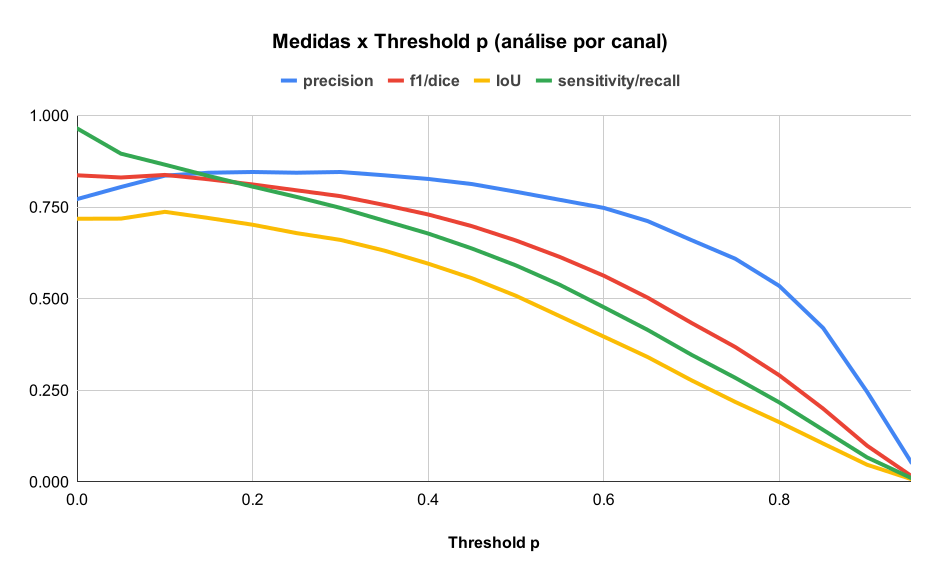
\includegraphics[width=0.8\textwidth]{figures/4_results/Medidas x Threshold p (análise por canal).png}
  
    \caption[Métricas obtidas na análise por canal.]{Precisão, \textit{f1-score}, Intersecção sobre União e sensibilidade em função do \textit{threshold} $p$ na análise por canal.}
    \label{fig:graphic-metrics-x-p-per-canal}
\end{figure}


%Verdadeiros positivos: 3087
%Falsos negativos: 451
%Falsos positivos: 649
%Acurácia: 0.7372820635299737
%Sensibilidade: 0.8725268513284341
%Precisão: 0.8262847965738758
%F1-Score: 0.8487764641187792


A Figura \ref{fig:marcacoes-final-canal} mostra a comparação entre máscaras geradas a partir da marcação manual do especialista e máscaras geradas pelo método com $p$=0,1. Já a Figura \ref{fig:marcacoes-final-canal-regioes} mostra algumas regiões ampliadas para melhor visualização dos detalhes das marcações.

Na Figura~\ref{fig:marcacoes-final-canal} é possível encontrar algumas regiões escuras na matriz óssea indicando que não foram marcados canais nestas regiões. Este é possivelmente um ponto a melhorar no método, e uma das possíveis causas para essas lacunas é o tamanho das manchas. Talvez utilizando sub-imagens com tamanho 640x640 não tenha sido possível atingir granularidade suficiente para cobrir toda a matriz óssea.

\begin{figure}[H]
    \center
    \begin{tabular}{@{}c@{}}
        \includegraphics[width=0.25\textwidth]{figures/4_results/204_mask_manual_lower_res.png}
        \\[\abovecaptionskip]
    \end{tabular}
    \begin{tabular}{@{}c@{}}
        \includegraphics[width=0.25\textwidth]{figures/4_results/204_net_mask_gaps_lower_res.png}
        \\[\abovecaptionskip]
    \end{tabular}
    \begin{tabular}{@{}c@{}}
        \includegraphics[width=0.25\textwidth]{figures/4_results/204_marcacao_rede_inteira_10.png}
        \\[\abovecaptionskip]
    \end{tabular}

    \begin{tabular}{@{}c@{}}
        \includegraphics[width=0.25\textwidth]{figures/4_results/302_mask_manual_lower_res.png}
        \\[\abovecaptionskip]
    \end{tabular}
    \begin{tabular}{@{}c@{}}
        \includegraphics[width=0.25\textwidth]{figures/4_results/302_net_mask_gaps_lower_res.png}
        \\[\abovecaptionskip]
    \end{tabular}
    \begin{tabular}{@{}c@{}}
        \includegraphics[width=0.25\textwidth]{figures/4_results/302_marcacao_rede_inteira_10.png}
        \\[\abovecaptionskip]
    \end{tabular}
  
    \caption[Comparação entre marcação manual feita por especialista e saída do método.]{Comparação entre marcação manual feita por especialista e saída do método. Na primeira coluna exemplos de marcações manuais; na segunda coluna as máscaras geradas pelo método utilizando um limiar $p$=0,1 com algumas lacunas destacadas em vermelho; na terceira coluna a imagem marcada a partir da máscara gerada pela rede.}
    \label{fig:marcacoes-final-canal}
\end{figure}

\begin{figure}[H]
    \center
    \begin{tabular}{@{}c@{}}
        \includegraphics[width=0.25\textwidth]{figures/4_results/204_r3c2_mask_manual_10.png}
        \\[\abovecaptionskip]
    \end{tabular}
    \begin{tabular}{@{}c@{}}
        \includegraphics[width=0.25\textwidth]{figures/4_results/204_r3c2_mask_net_10.png}
        \\[\abovecaptionskip]
    \end{tabular}
    \begin{tabular}{@{}c@{}}
        \includegraphics[width=0.25\textwidth]{figures/4_results/204_r3c2_net_out_10.png}
        \\[\abovecaptionskip]
    \end{tabular}

    \begin{tabular}{@{}c@{}}
        \includegraphics[width=0.25\textwidth]{figures/4_results/204_r4c2_mask_manual_10.png}
        \\[\abovecaptionskip]
    \end{tabular}
    \begin{tabular}{@{}c@{}}
        \includegraphics[width=0.25\textwidth]{figures/4_results/204_r4c2_mask_net_10.png}
        \\[\abovecaptionskip]
    \end{tabular}
    \begin{tabular}{@{}c@{}}
        \includegraphics[width=0.25\textwidth]{figures/4_results/204_r4c2_net_out_10.png}
        \\[\abovecaptionskip]
    \end{tabular}
  
    \caption[Comparação de regiões ampliadas das marcações manuais feita por especialista e de saídas do método]{Comparação de regiões ampliadas das marcações manuais feita por especialista e de saídas do método. Na primeira coluna regiões ampliadas de marcações manuais, na segunda coluna as respectivas regiões nas máscaras geradas pelo método utilizando um limiar $p$=0,1, e na terceira coluna as respectivas regiões na imagens marcadas a partir das máscaras geradas pela rede.}
    \label{fig:marcacoes-final-canal-regioes}
\end{figure}

\subsection{Comparação}

A fim de comparação, foi feita uma implementação do algoritmo proposto por \cite{gondim2021automatic} utilizando a linguagem de programação Python na versão 3.10. As imagens de lâmina inteira do conjunto de testes foram então segmentadas e foi realizada a análise por canal conforme descrito anteriormente. A Figura \ref{fig:intersection-gondim} mostra exemplos de componentes conectados obtidos na análise por canal do algoritmo.


\begin{figure}[H]
    \centering
    
    \begin{tabular}{@{}c@{}}
        \includegraphics[width=0.6\textwidth]{figures/4_results/components/gondim_203_component_1.png} \\
        \includegraphics[width=0.6\textwidth]{figures/4_results/components/gondim_204_component_1.png} \\
        \includegraphics[width=0.6\textwidth]{figures/4_results/components/gondim_301_component_1.png} 
    \end{tabular}

    \caption[Exemplos de componentes conectados obtidos pelo método proposto por \cite{gondim2021automatic}.]{Três exemplos de componentes conectados analisados. Na primeira coluna o componente na máscara de referência (padrão ouro). Na segunda coluna a segmentação do algoritmo de \cite{gondim2021automatic} para o respectivo componente. Na terceira coluna a intersecção entre a primeira e a segunda coluna.}
    \label{fig:intersection-gondim}
\end{figure}

Foi observado que no método proposto neste trabalho era menos comum a aparição de falsos negativos. Além disso, algumas imagens do conjunto de testes apresentavam concavidades no formato da matriz óssea e o método de \cite{gondim2021automatic} não reagiu bem para tais imagens, conforme mostrado na Figura \ref{fig:gondim-bad-prediction}.

\begin{figure}[H]
    \centering
    
    \begin{tabular}{c}
        \includegraphics[width=0.8\textwidth]{figures/4_results/falha-gondim_lower_res.png} \\[\abovecaptionskip]
    \small (a) 
    \end{tabular}

    \caption[Exemplo de falha do algoritmo proposto por \cite{gondim2021automatic}.]{Exemplo de falha do algoritmo proposto por \cite{gondim2021automatic}. Apesar de funcionar para imagens com matriz óssea em um formato convexo (sub-figuras (a) e (b)) o método falha ao trabalhar com imagens que apresentem concavidades na matriz óssea (sub-figuras (c) e (d)).}
    \label{fig:gondim-bad-prediction}
\end{figure}

Os resultados obtidos em \cite{gondim2021automatic} mostram acurácia e especificidade próximas a 96\%, sensibilidade acima de 80\% e cerca de 90\% de \textit{f1-score}. Porém as marcações dos especialistas não seguiram a forma exata das estruturas, assim, foram considerados como verdadeiros positivos os canais cuja marcação do especialista estivesse ao menos 20\% contida na marcação feita pelo método. 

Não fica claro se as imagens utilizadas em \cite{gondim2021automatic} continham imagens de diferentes regiões da diáfise femoral -- região intermediária do fêmur. Devido à anatomia do osso, imagens provenientes da região central da diáfise resultam em uma matriz óssea mais arredondada, semelhante à Figura \ref{fig:gondim-bad-prediction}(a), enquanto cortes mais próximos às extremidades da diáfise podem resultar em imagens cuja matriz óssea apresenta outros formatos, como o observado na Figura \ref{fig:gondim-bad-prediction}(c). 

A análise por canal -- descrita na seção 4.2 -- da reprodução do algoritmo proposto por \cite{gondim2021automatic} apresentou um \textit{f1-score} de aproximadamente 17,5\% e uma Intersecção sobre União de 9,6\%. A Tabela \ref{tab:metricas-comparacao-por-canal} mostra os resultados obtidos pela análise por canal para cada um dos métodos. Vale ressaltar que esse valor é bem inferior ao obtido pelos autores pois neste trabalho são consideradas como válidas as intersecções que coincidem 70\% ou mais com o canal da máscara de referência, enquanto que no trabalho original era consideradas interseções de apenas 20\%.

%Verdadeiros positivos: 391
%Verdadeiros negativos: 3447
%Falsos positivos: 241
%Acurácia: 0.09585682765383673
%Sensibilidade: 0.10187597707139134
%Precisão: 0.6186708860759493
%F1-Score: 0.1749440715883669
%Jaccard: 0.095

% TABELA AQUI
\begin{table}[h]
\center
\begin{tiny}
\begin{tabular}{|l|l|l|l|l|}
\hline
\rowcolor[HTML]{C0C0C0} 
\textbf{Método} & \textbf{Precisão} & \textbf{F1-Score} & \textbf{Sensibilidade}   & \textbf{IoU}     \\ 
\hline
\cellcolor[HTML]{EFEFEF}\textbf{FCN ($p$ = 0.10)} & 0.826 & 0.849 & 0.872 & 0.737 \\
\hline
\cellcolor[HTML]{EFEFEF}\textbf{Algoritmo \cite{gondim2021automatic}} & 0.619 & 0.175 & 0.102 & 0.095 \\
\hline
\end{tabular}
\end{tiny}
\caption{Médias de precisão, \textit{f1-score}, sensibilidade e Intersecção sobre União para cada os métodos de segmentação testados.}
    \label{tab:metricas-comparacao-por-canal}
\end{table}